% !TEX encoding = UTF-8

\documentclass[a4paper,12pt]{article}
\usepackage[T1]{fontenc}
\usepackage[utf8]{inputenc}
\usepackage[italian]{babel}
\usepackage{graphicx}
\usepackage{color, colortbl}
\definecolor{Ash}{rgb}{0.7,0.75,0.71}


\begin{document}

\title{\textbf{TrackMyCar - Live Positioning System} \\ Documento di Vision}

\author{Kevin Mansoldo, Matteo Dal Monte, Luca Vicentini}
\date{30 Giugno 2015}
\maketitle
\pagebreak

\tableofcontents
\pagebreak

\section{Lista Destinatari del Documento}

\begin{table*}[ht]
\begin{center}
\begin{tabular}{p{1cm} p{4.5cm} p{3.5cm} p{3.5cm}}
\rowcolor{Ash}
\hline
Copia & Persona & Organizzazione & 30 Giugno 2015 \\ \hline
1 & Kevin Mansoldo & Azienda & 30 Giugno 2015 \\ 
2 & Matteo Dal Monte & Azienda & 30 Giugno 2015 \\ 
3 & Luca Vicentini & Azienda & 30 Giugno 2015 \\ 
4 & Claudio Tomazzoli & Cliente & 30 Giugno 2015 \\ \hline
\end{tabular}
\end{center}


\begin{center}
\begin{tabular}{p{6cm} p{3.5cm} p{3.5cm}}
\rowcolor{Ash}
\hline
Azione & Persona & Data \\ \hline
Documento redatto da & Kevin Mansoldo & 30 Giugno 2015 \\ 
Documento approvato da & Matteo Dal Monte & 30 Giugno 2015 \\ 
Documento approvato da & Luca Vicentini & 30 Giugno 2015 \\ \hline
\end{tabular}
\end{center}
\end{table*}

\subsection{Versione Documento}
\begin{table*}[ht]
\begin{center}
\begin{tabular}{p{1cm} p{3cm} p{5cm} p{3.5cm}}
\rowcolor{Ash}
\hline
Versione & Autore & Note & Data \\ \hline
1.0 & Kevin Mansoldo & Stesura Iniziale & 8 Giugno 2015 \\ 
1.1 & Kevin Mansoldo & Revisione su osservazioni del gruppo & 17 Giugno 2015 \\ 
1.2 & Kevin Mansoldo & Revisione Finale & 30 Giugno 2015 \\ \hline
\end{tabular}
\end{center}
\end{table*}

\subsection{Supporto Documento}
\begin{table*}[ht]
\begin{center}
\begin{tabular}{p{6cm} p{5cm} p{2cm}}
\rowcolor{Ash}
\hline
Nome File & Tipo & Estensione \\ \hline
Vision & Portable Document Format & .pdf \\ \hline
\end{tabular}
\end{center}
\end{table*}

\clearpage

\pagebreak


\section{Introduzione e Obiettivi}

Lo scopo del sistema che si vuole implementare è quello di poter tracciare in tempo reale il o i veicoli collegati in caso di furto o smarrimento. Tramite un'interfaccia visuale è possibile tenere sotto controllo la posizione, la velocità e lo storico dei percorsi effettuati. Inoltre viene fornita la possibilità di sfruttare l'integrazione con sistemi di videosorveglianza interni al veicolo, identificando così eventuali malintenzionati. 

L'applicazione, dotata di una intuitiva interfaccia grafica, permette quindi la rapida fruizione dei contenuti tramite semplici menu contestuali.



\section{Definizioni, Acronimi e Abbreviazioni}

Per le definizioni di alcuni termini fondamentali, fare riferimento al glossario ``Glossario.pdf'' all'interno della documentazione di progetto.

\begin{table}[h]
\begin{center}
\begin{tabular}{ l  l  l } 
\rowcolor{Ash}	
\hline	
Nome File & Tipo File & Estensione  \\ \hline
Development Case & Linee guida di sviluppo del progetto & DevCase.pdf  \\ 
Glossario & Descrizione di termini specifici & Glossario.pdf  \\ \hline
\end{tabular}
\end{center}
\end{table}

\pagebreak

\section{Panoramica}
L'attuale funzionamento degli antifurti non prevede un tracciamento dell'abitacolo in tempo reale, ma solamente con emissione di segnale acustico nella speranza di far desistere il malintenzionato. 

La soluzione è l'installazione di un dispositivo multifunzione che si interfacci con molteplici moduli di comunicazione nel tentativo di fornire informazioni sulla posizione del veicolo in tempo reale, con la massima precisione possibile. Inoltre, può essere installato un sistema di videosorveglianza a circuito chiuso.
Questo prodotto è utile e permette di tenere sotto controllo la propria vettura in caso di furto.

\begin{table}[h]
In sintesi:
\begin{center}
\begin{tabular}{ p{4 cm}  p{9 cm} }
\hline	
Il problema di & Controllare e tracciare la propria vettura \\ \hline
Interessa & Privati e Aziende \\ 
Il cui impatto è & Economico \\ 
Una soluzione sarebbe & Non muoversi da casa!!!  \\ 
& TrackMyCar \\ \hline
\end{tabular}
\end{center}
\end{table}

\begin{table}[h]
Utilizzatori del prodotto:
\begin{center}
\begin{tabular}{ p{4 cm}  p{9 cm} }
\hline	
Chi & Coloro che possiedono uno o più veicoli \\ \hline
Per & Tracciare e controllare il veicolo in tempo reale \\ 
TrackMyCar & Software per rintracciare i veicoli in caso di furto \\ 
Che & Assicura la tranquillità dell'utente finale, \\
&semplificando controllo e recupero \\ 
Diversamente da & Iniziative personali (recupero autonomo veicolo) \\ 
&Altri prodotti di terze parti \\ \hline
\end{tabular}
\end{center}
\end{table}

\pagebreak

\subsection{Perchè utilizzare questo prodotto?}
Un sistema di tracciamento in tempo reale come TrackMyCar si distingue dai diretti concorrenti per semplicità di utilizzo e ricchezza di informazioni consultabili in diretta.

Il proprietario dei veicoli potrà monitorare costantemente svariate informazioni, indicando tempestivamente eventuali anomalie. La comunicazione avviene mediante un modulo GPS e uno per la connessione dati, entrambi integrati nella centralina di controllo. Sarà dunque possibile valutare posizione, velocità e percorso di ciascun veicolo iscritto all'interno del sistema, nonchè video provenienti direttamente dall'abitacolo.

Le caratteristiche citate permettono di ridurre drasticamente i tempi di recupero dei propri veicoli in caso di furto, avendo accesso immediato a qualunque informazione utile, in modo semplice e diretto, a tutela del proprio investimento.



\section{Parti interessate e Attori del sistema}

\begin{table}[h]
Parti interessate:
\begin{center}
\begin{tabular}{ p{2 cm}  p{7 cm}  p{4 cm} }
\rowcolor{Ash}	
\hline	
Stakeholder & Descrizione & Responsabilità \\ \hline
User & Utente finale che usufruisce del servizio & Guidatore\\ 
Admin & Controllo e Gestione & Deve garantire il corretto funzionamento del sistema \\ 
 &  & Responsabile del sistema \\ \hline
\end{tabular}
\end{center}
\end{table}

\begin{table}[h]
Attori del sistema:
\begin{center}
\begin{tabular}{ p{2 cm}  p{7 cm}  p{4 cm} }
\rowcolor{Ash}	
\hline	
Nome & Descrizione & Stakeholder \\ \hline
Admin & Proprietario Veicolo & Proprietario Auto \\ 
Regular User & Utilizzatore del veicolo & Guidatore di Turno \\ \hline
\end{tabular}
\end{center}
\end{table}

\pagebreak

\section{Requisiti}
I requisiti rappresentano elementi fondanti della progettazione, in quanto se venissero violati, porterebbero al fallimento dello scopo stesso di creazione del prodotto. Essi si dividono in funzionali e non funzionali.

\begin{table}[h]
Business Needs:
\begin{center}
\begin{tabular}{ p{6,5cm}  p{6,5cm} }
\rowcolor{Ash}	
\hline	
Nome & Descrizione \\ \hline
Localizzazione & Posizione attuale del veicolo \\ 
Tracciamento & Percorso in tempo reale \\ 
Allarmi & Notifiche per eventi anomali \\ 
Avvisi & SMS o mail con posizione attuale veicolo \\ 
Storico & Raccolta percorsi effettuati \\ 
Video & Identificazione malintenzionati da abitacolo \\ \hline
\end{tabular}
\end{center}
\end{table}

\begin{table}[h]
Requisiti Utente:
\begin{center}
\begin{tabular}{ p{6,5cm}  p{6,5cm} }
\rowcolor{Ash}	
\hline	
Nome & Descrizione \\ \hline
Configurazione & Attivazione immediata della comunicazione dal dispositivo \\ 
Gestione Utenze & Creazione, aggiornamento e cancellazione account spettano all'amministratore di sistema \\ 
Gestione Veicoli & Associazione Veicolo-Percorso-Informazioni \\ 
Gestione Accessi &  Aree Riservate distinte per gli utenti (admin o regular) \\ 
Notifiche &  SMS/mail al verificarsi di particolari eventi (furto o violazioni)\\ \hline
\end{tabular}
\end{center}
\end{table}

\pagebreak

\section{Concetto Operativo}
\begin{figure}[ht]
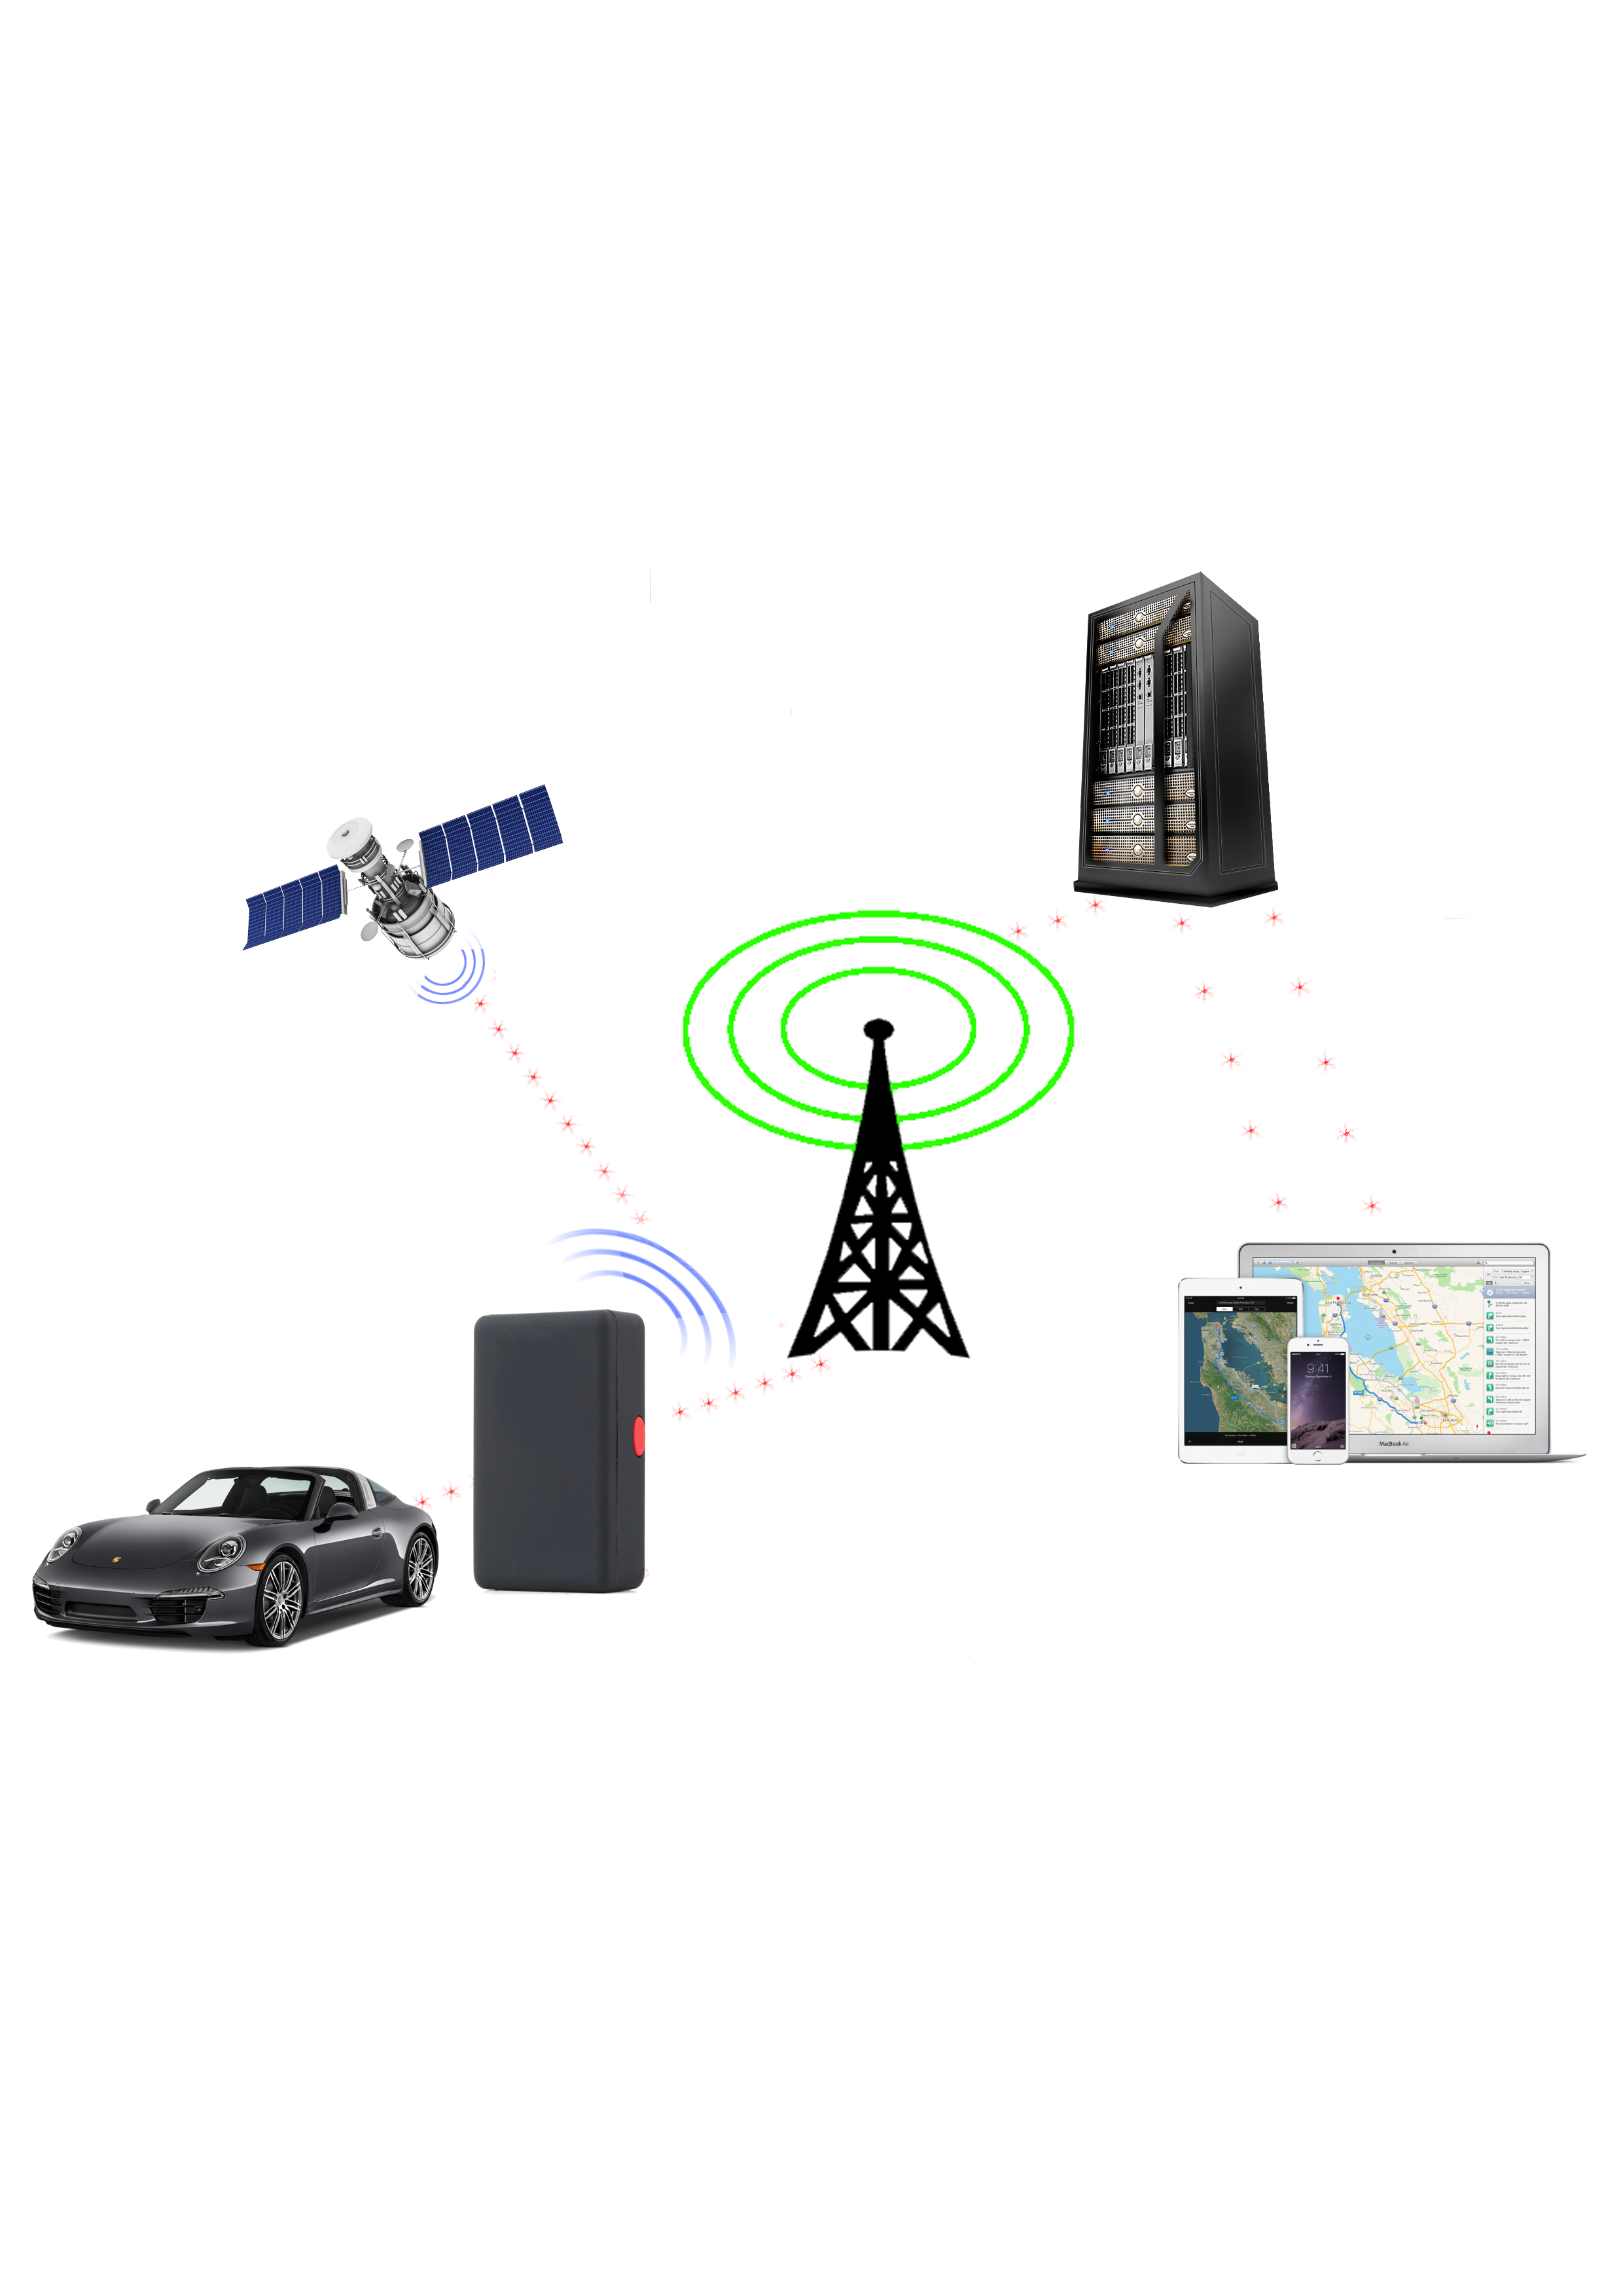
\includegraphics[trim={0 6cm 0 6cm}, clip, scale=.75]{Concetto2.png}
\caption{Schema di funzionamento del sistema considerato.}
\end{figure}
\end{document}